\documentclass[]{standalone}

\begin{document}
	\begin{frame}{Tissue Segmentation}{A Gaussian Mixture model approach.}
	
	\vspace{-25pt}
		\begin{columns}
			\begin{column}{0.60\textwidth}
			\small
				\begin{itemize}
				\item \textbf{Find Tissues Mean Values and Weights:} Starting from the atlas' partial volume maps compute the mean pixel value and the the fraction of pixels belonging to each tissue;
				\item \textbf{Define a Gaussian Mixture Model:} A mixture of three Gaussian distributions is defined starting from the parameters found;
				\item \textbf{Expectation Maximization:} An expectation maximization algorithm finds the best parameters of the Gaussian mixture model;
				\item \textbf{Classification:} Each pixel is classified.
				\end{itemize}
			\end{column}
			\begin{column}{0.40\textwidth}
			\begin{figure}[h!]
			\centering
			\vspace{-6pt}

				\begin{subfigure}{0.4\textwidth}
					\centering
					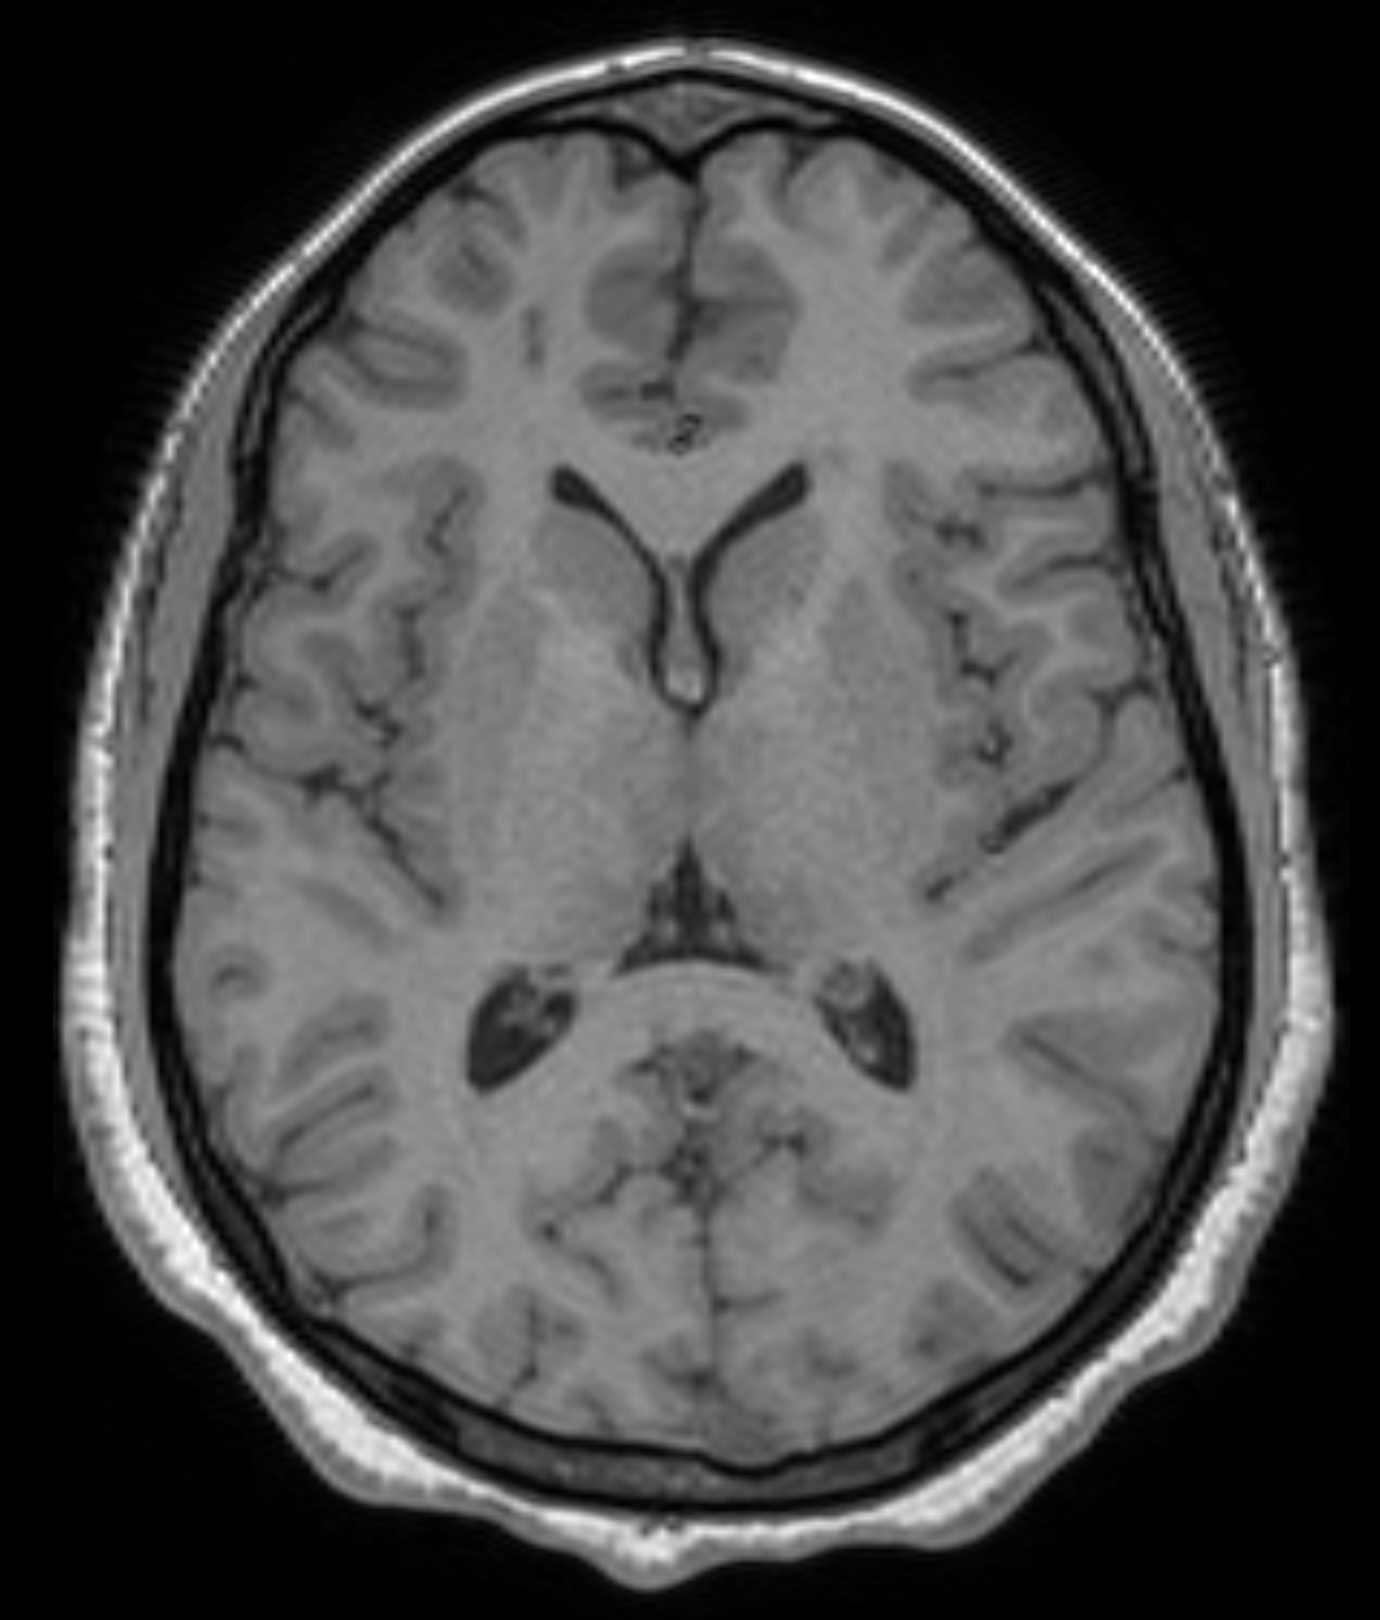
\includegraphics[scale=0.05]{./IMG/T1.jpg}
				\end{subfigure}
				\hspace{10pt}
				\begin{subfigure}{0.4\textwidth}
					\centering
					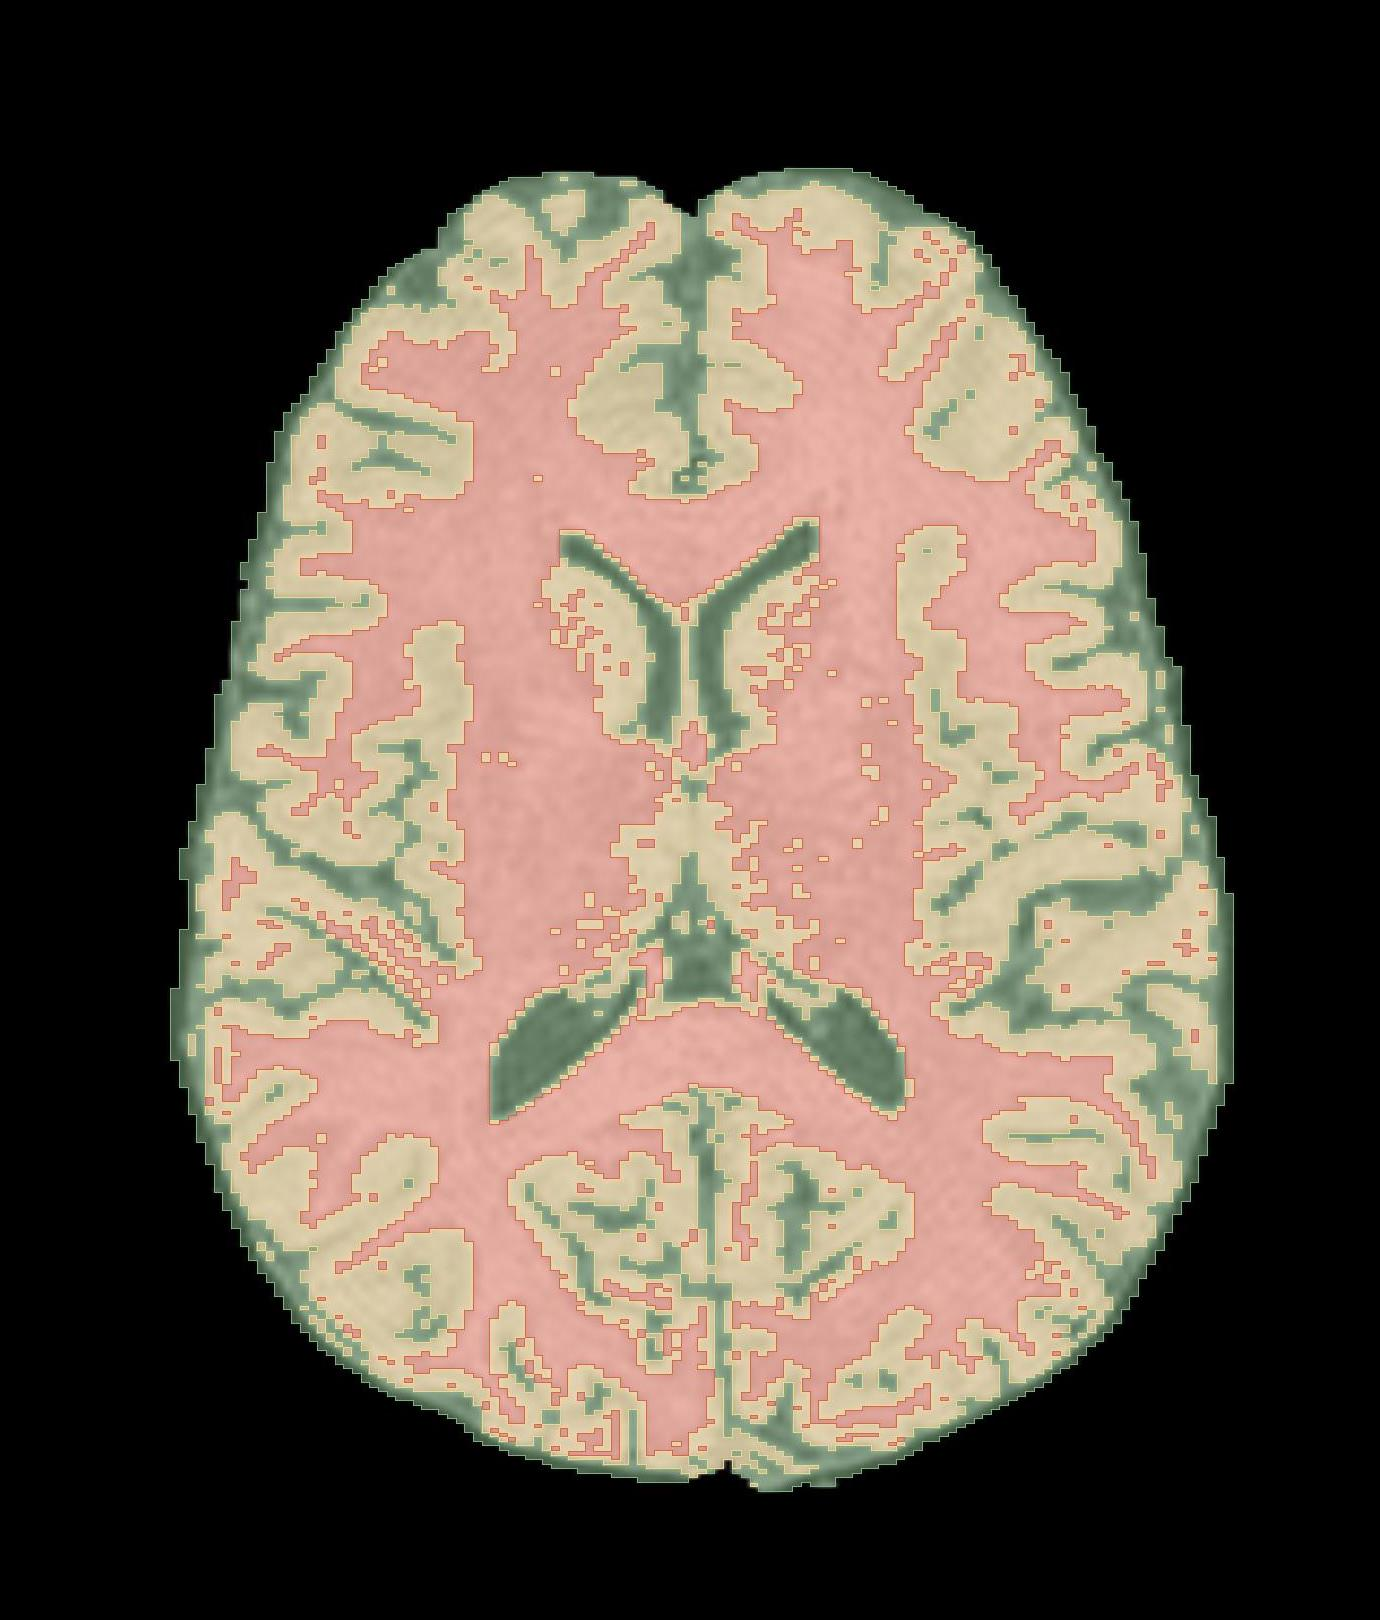
\includegraphics[scale=0.05]{./IMG/segmented_axial.jpg}
				\end{subfigure}

				\begin{subfigure}{0.4\textwidth}
					\centering
					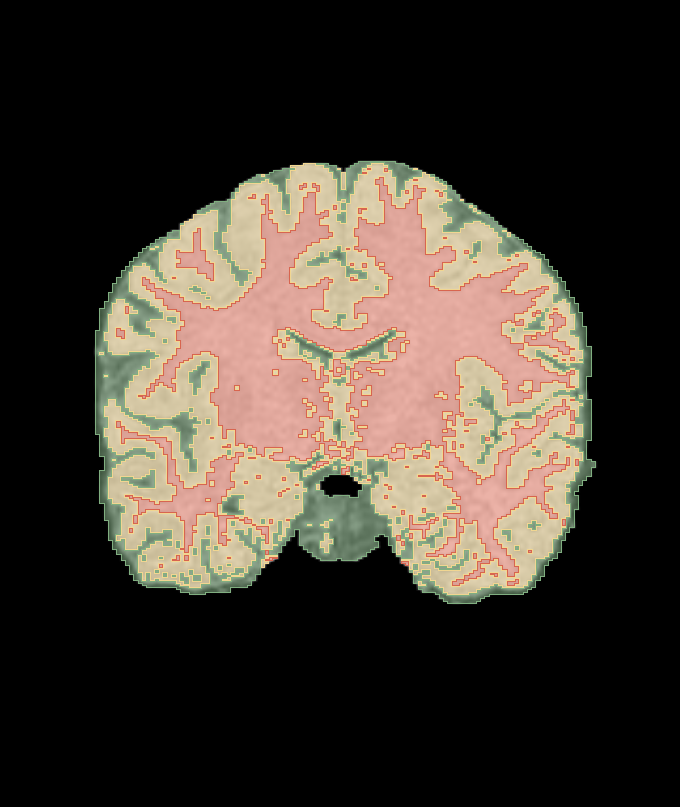
\includegraphics[scale=0.102]{./IMG/segmented_frontal.png}
				\end{subfigure}
				\hspace{10pt}
				\begin{subfigure}{0.4\textwidth}
					\centering
					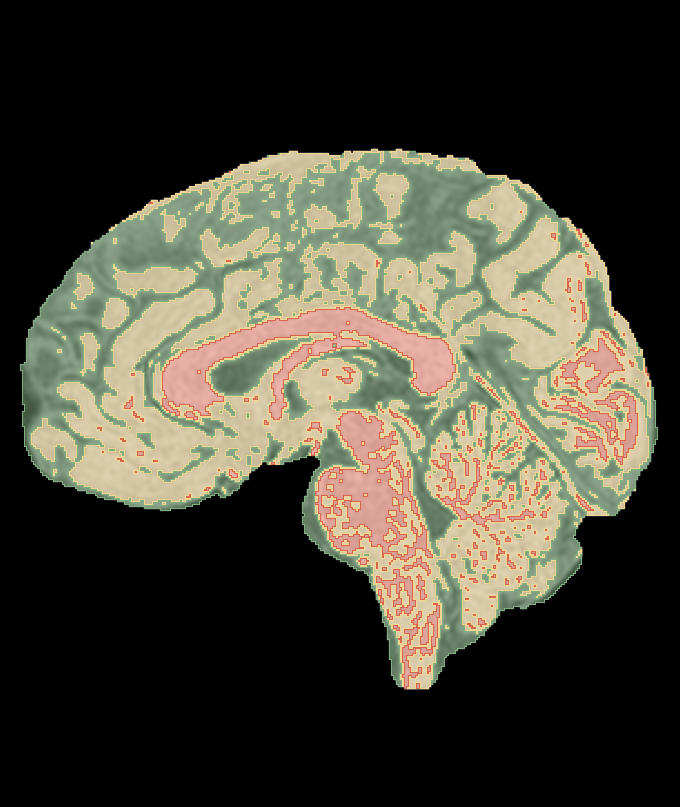
\includegraphics[scale=0.102]{./IMG/segmented_lateral.png}
				\end{subfigure}
				\hspace{10pt}
			\end{figure}
			\end{column}
		\end{columns}
	\end{frame}
\end{document}
